\chapter{序論}
\label{chap_intro}

% 英語で言うところのイントロダクションです。通常、「序論」(introduction)で始める場合は「結論」(conclusion)という章で締めます。もし「はじめに」で始まる場合は「おわりに」です。

% この章では研究の背景や課題などを簡潔に説明します。2から4ページもあれば十分ですし、細かく節に分ける必要もありません。この章で必要なことは、なぜこの論文が書かれたのか、過去の研究に対する位置付け・課題は何か、この研究でどこまでを明らかにしようとしているのかを少ないページ数で説明することです。

% このような序論の存在しない修士論文はたくさん存在しますが、何十ページにもなる修士論文では研究の位置付けや課題がどこに書かれているのか読者は見失いやすくなります。先頭に独立した章で簡潔に道筋を示すことで、続く章を読者が読みやすくなります。

\section{素粒子標準模型}
\label{sec_intro_sm}

\section{標準模型を超える物理}
\label{sec_intro_bsm}

\section{LHC-ATLAS実験}
\label{sec_intro_atlas}

ジュネーブに拠点を置く欧州原子核研究機構(CERN)では超対称性粒子をはじめとする新粒子探索や素粒子標準模型の精密を目的にLHC-ATLAS実験を行なっている。
LHCとはスイスとフランスの国境付近、地下100mに建設された周長26.7 kmに及ぶ陽子陽子衝突型加速器である(図\ref{LHCoverview})。LHCには8つの地下と地上をつなぐトンネルがあり、それぞれPoint1からPoint8と名付けられている。このうち4つのPointで陽子陽子衝突が行われ、各衝突点でそれぞれ特徴の異なる検出器を用いた独立した実験が進行している。本研究はその中の一つであるA Toroidal LHC ApparatuS (ATLAS)実験に関するものである。
LHC加速器内では、陽子が約$10^{11}$個ずつの束にまとめられ、バンチ構造を形成している。LHCを周回しながら、最大エネルギー7\,TeVまで加速され、各衝突点で40.079\,MHzの頻度で衝突が起こる。

\begin{figure} 
\centering
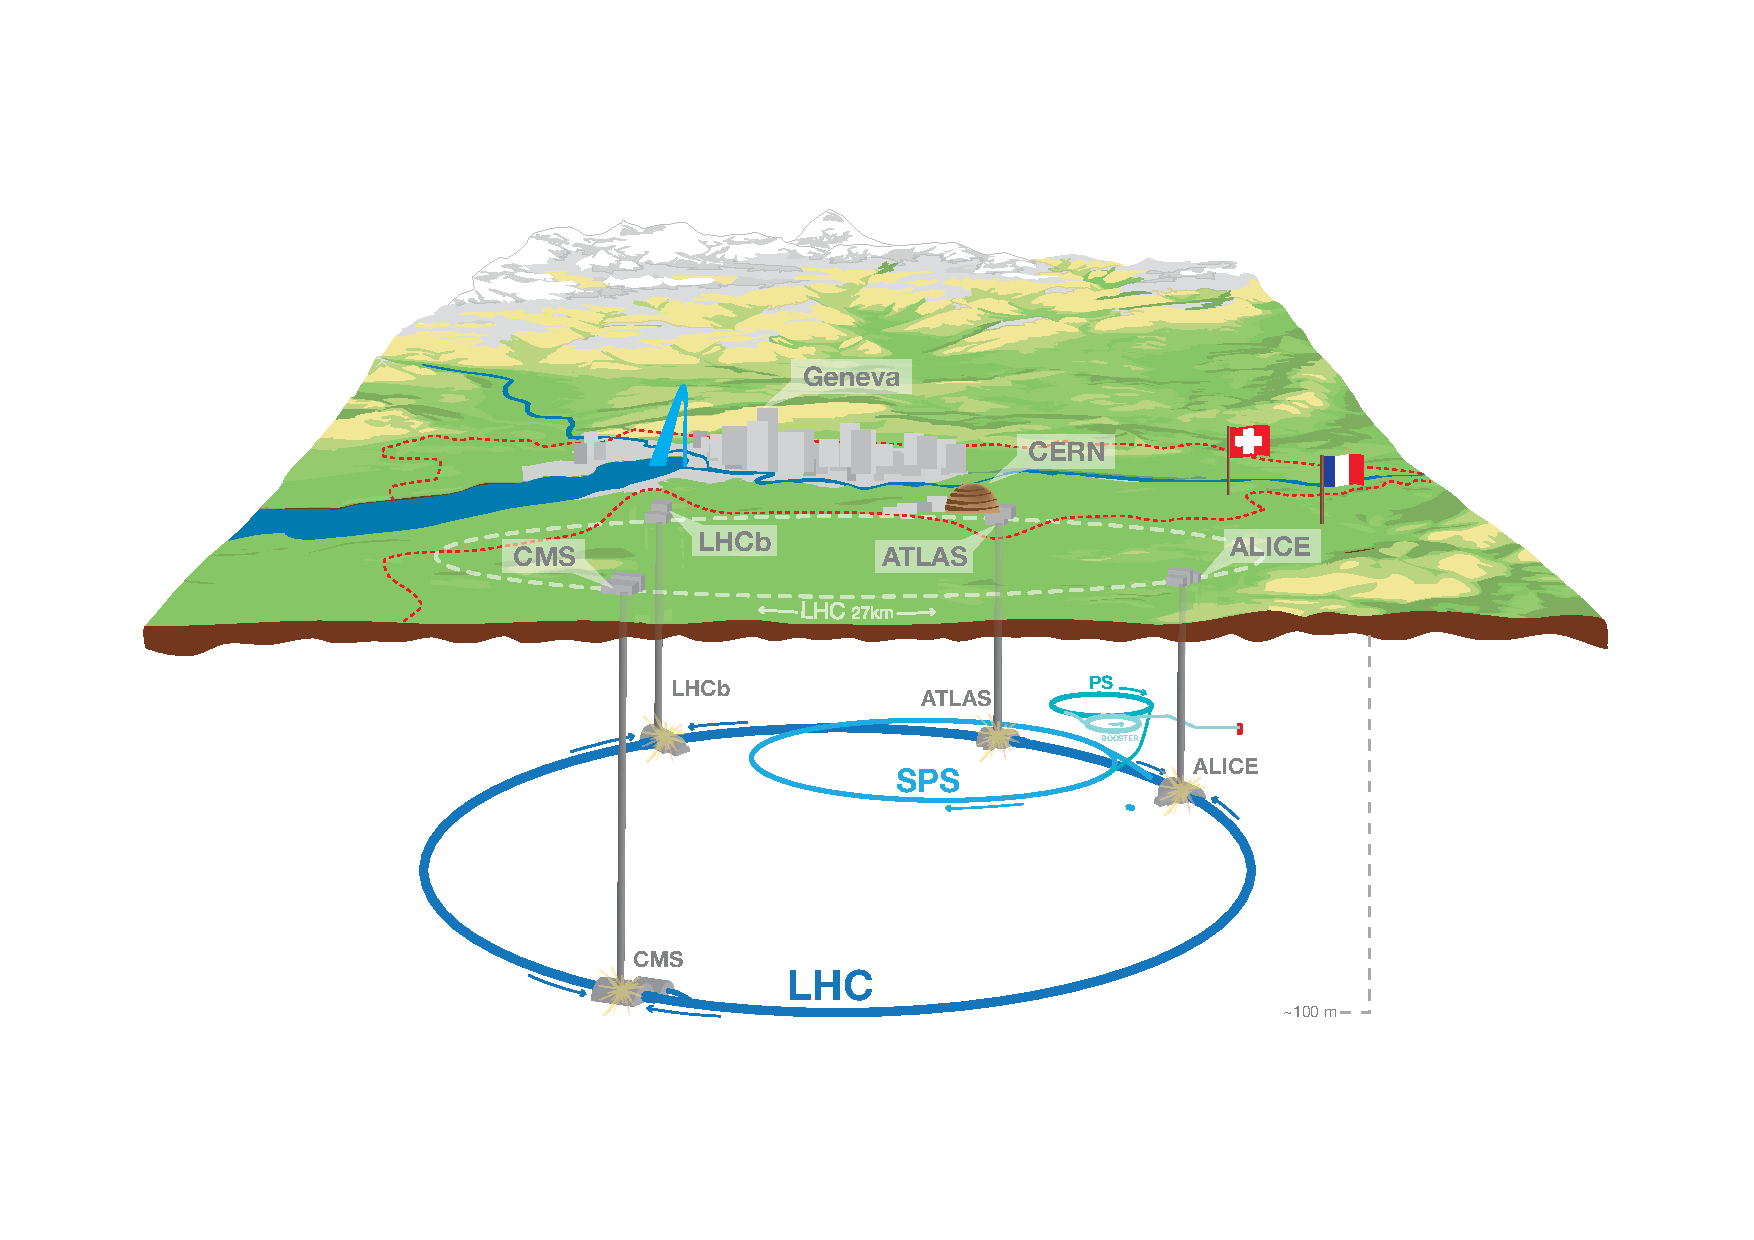
\includegraphics[width=16cm]{fig/Intro/LHCoverview.pdf}
\caption[LHC 加速器の概観]{LHC 加速器の概観\cite{cern_general_photo}}
\label{LHCoverview}
\end{figure}

ATLAS(A Toroidal LHC Apparatus)検出器は複数の検出器で構成された大型汎用検出器である。図\ref{ATLASdetector}に全体像を示す。ATLAS検出器は主に内部飛跡検出器、カロリメーター、ミューオンスペクトロメーターという3つの検出器群から成り立っている。最内層に設置された内部飛跡検出器はソレノイド磁石を使用して、荷電粒子の飛跡を再構成し、運動量を測定する。その外側に配置された電磁カロリメーターとハドロンカロリメーターでは、それぞれ電子、光子およびハドロンのエネルギーを測定する。最外層にあるミューオンスペクトロメーターでは内側の検出器を透過してきたミューオンを捉え、トロイダル磁石を使用してその運動量を測定する。本研究のテーマであるミューオンスペクトロメーターについては\ref{}節で詳しく説明する。

\begin{figure} 
    \centering
    \includegraphics[width=16cm]{fig/Intro/ATLASdetector.pdf}
    \caption[ATLAS検出器の概要]{ATLAS検出器の概要図\cite{JINST:2008}}
    \label{ATLASdetector}
\end{figure}

LHC-ATLAS実験では陽子陽子衝突が40 MHzで行われ、1回のバンチ衝突ごとに約10\,Mb程度の信号が生じる。これは1秒間に約1\,Pbpsのデータ量に相当し、これらの全てのデータをストレージに転送し、保存することは技術的に不可能である。一方、陽子陽子衝突で生じるほとんどの事象は非弾性散乱など物理解析にとって興味の薄いものである。実際にATLAS実験で測定された各物理過程の反応断面積を図\ref{LHCcrosssection}に示す。pp→Xで示された陽子衝突の断面積に比べて、pp→Hで示されるヒッグス生成事象の断面積はO($10^10$)倍小さい。このような莫大な背景事象の中から、興味のある事象のみを選別し保存するシステムをトリガーシステムと呼ぶ。
新粒子探索や標準模型の精密測定の多くの解析において、統計量はその解析感度を決定する重要な要素である。ATLAS実験において、より洗練されたトリガーシステムを構築し、興味のある物理事象への感度を高めていくことは、物理探索に直結する重要な課題である。\par

\begin{figure} 
    \centering
    \includegraphics[width=16cm]{fig/Intro/LHCcrosssection.pdf}
    \caption[陽子陽子衝突における各反応事象の断面積]{陽子陽子衝突における各反応事象の断面積 \cite{atlas_phys_pub_hllhc}}
    \label{LHCcrosssection}
\end{figure}


\section{高輝度LHC実験に向けたPhase-\two アップグレード}
\label{sec_intro_phase2upgrade}

\begin{figure} 
\centering
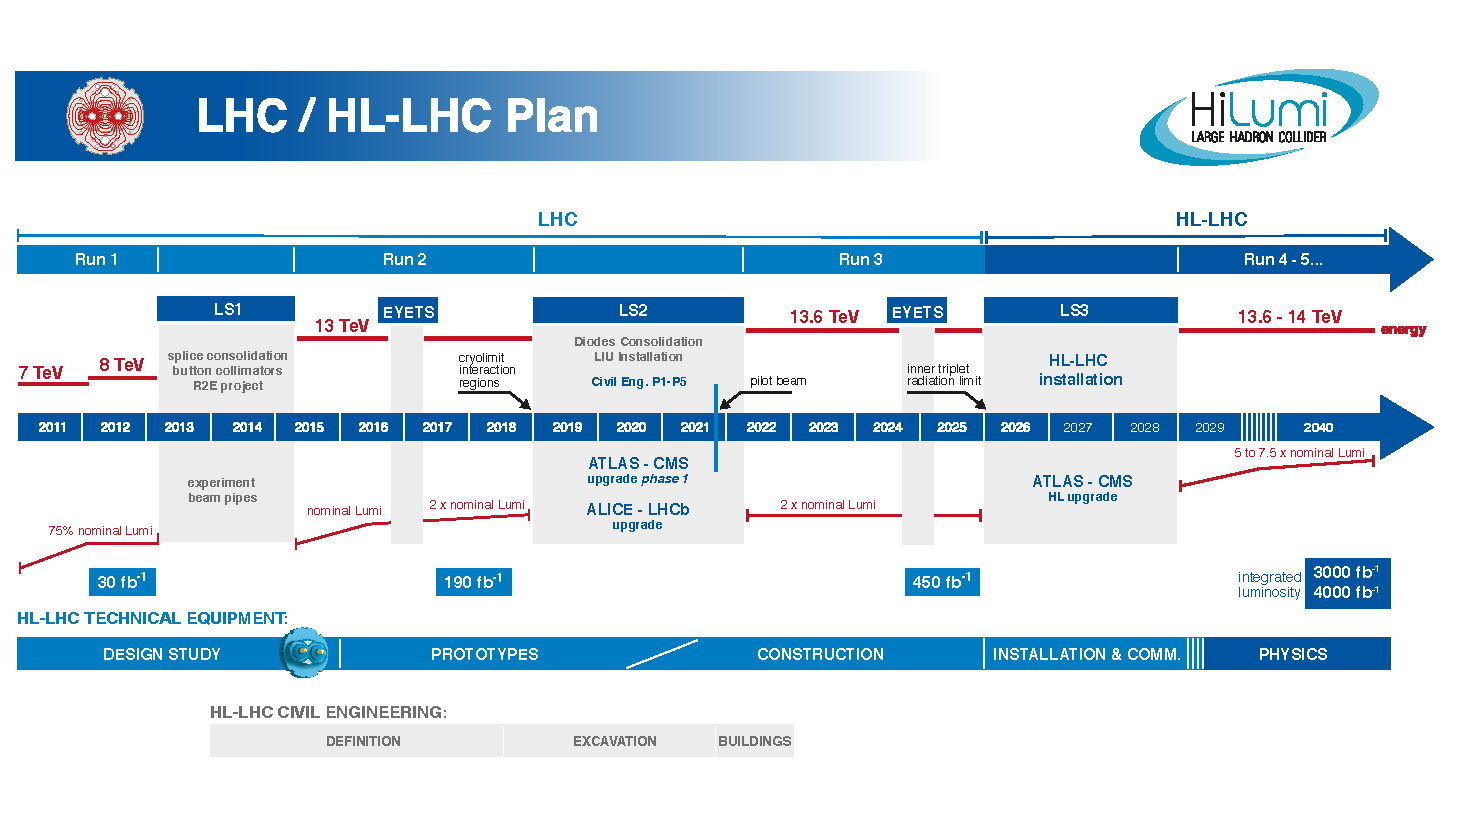
\includegraphics[width=16cm]{fig/Intro/LHCschedule.pdf}
\caption[LHC実験のスケージュール]{LHC実験のスケジュール\cite{cern_hllhc_industry}}
\label{LHCschedule}
\end{figure}

LHC実験は2010年から本格的に稼働を開始し、2024年現在、第三期運転(Run3)が進行中である。Run3では2025年までに累計450\,$\mathrm{fb}^{-1}$の統計量が蓄積することが予定されている。その後、3年間のLong Shutdown(LS3)を経てLHC実験は高輝度LHC実験に大幅にアプグレードされる。高輝度LHC実験では瞬間最高ルミノシティが現在のの$2\times10^{34}\,\mathrm{cm}^{-2}\mathrm{s}^{-1}$から$5 \text{~} 7.5\times10^{34}\,\mathrm{cm}^{-2}\mathrm{s}^{-1}$に増強され、2040年の実験終了までに3000 ~ 4000\,$\mathrm{fb}^{-1}$の統計量が貯められる予定である。一方で、高輝度LHC実験では瞬間ルミノシティの増加に伴い、一回のバンチ衝突ごとに発生する陽子陽子衝突数(パイルアップ)が増加し、背景事象が大幅に増加する。高輝度環境下で背景事象を適切に削減し、興味のある事象だけを効率的に取得するためには検出器やトリガーシステムのアップグレードが不可欠である。\par

図\ref{Ptthreshold}に高輝度LHC実験で現行のトリガーシステム(特に電子やミューオンの横方向運動量をもとに閾値を設定するシングルレプトントリガーシステム)を利用した場合の各物理事象へのアクセプタンスの見積を表す。現行のレプトンの運動量分解能や信号転送レートを維持したまま、信号事象や背景事象が増加すると、閾値を超えるレプトンの数が読み出し能力を超えるため、レプトンの横方向運動量閾値を50 GeV程度まで上げなくてはならない。しかし、トリガーシステムをアップグレードすることで運動量分解能を向上し、読み出し能力を増強すれば横方向運動量閾値を20 GeVまで低く抑えることができる。これにより、例えば、終状態に低運動量レプトンが生成される縮退したSUSY粒子の崩壊事象へのアクセプタンスは約4倍に増幅されることが見込まれる。


\begin{figure} 
\centering
\includegraphics[width=16cm]{fig/Intro/Ptthreshold.pdf}
\caption[高輝度LHC-ATLAS実験の主なターゲットとなる事象における、レプトンの pT 閾値とアクセプタンスの関係]{高輝度LHC-ATLAS実験の主なターゲットとなる事象における、レプトンの pT 閾値とアクセプタンスの関係\cite{tdr_phase2tdaq_2017020}}
\label{Ptthreshold}
\end{figure}

\section{本論文の目的・内容と構成}
\label{sec_intro_purpose}





